\documentclass[conference]{IEEEtran}
\usepackage{amsmath,amssymb,amsthm}
\usepackage{graphicx}
\usepackage{booktabs}
\usepackage{cite}
\usepackage[hidelinks]{hyperref}
\graphicspath{{figures/}}
\pdfminorversion=4

\newtheorem{proposition}{Proposition}
\newcommand{\bv}[1]{\mathbf{#1}}
\newcommand{\Jm}{\boldsymbol{\mathcal{J}}}

\begin{document}

\title{Modeling and Passivity-Based Current Control of a 2~MW Direct-Drive PMSG Wind Energy Conversion System}

\author{
\IEEEauthorblockN{Said Regani}
\IEEEauthorblockA{\textit{L2EI Laboratory}\\
\textit{Jijel University}\\
BP 98 Ouled Aissa, Jijel 18000, Algeria}
\and
\IEEEauthorblockN{Manal Messadi}
\IEEEauthorblockA{\textit{L2EI Laboratory}\\
\textit{Jijel University}\\
BP 98 Ouled Aissa, Jijel 18000, Algeria}
\and
\IEEEauthorblockN{Kemih Karim}
\IEEEauthorblockA{\textit{L2EI Laboratory}\\
\textit{Jijel University}\\
BP 98 Ouled Aissa, Jijel 18000, Algeria}
}

\maketitle

\begin{abstract}
This paper presents the modeling of a 2~MW direct-drive wind energy conversion system based on a
permanent magnet synchronous generator (PMSG), including the turbine aerodynamics, the generator, the
back-to-back converter, the DC link, the $L$ filter and the grid, and the design of a passivity-based
current controller for the machine-side converter. The generator is described in the receptor
convention with parameters taken from published data, and the consistency of all the signs of the
model is verified by an exact power balance between the aerodynamic power, the stored energy, the
losses and the power injected into the grid. A step and a turbulent wind profile are defined for the
evaluation of the system. The passivity-based controller keeps the workless coupling of the machine
model and injects damping; its stability is proven with a storage function. Simulations with a
sampling period equal to half of the switching period and a one-sample computation delay give a rise
time of 3~ms without overshoot, a cross-coupling below 0.5\,\% of the reference step and a zero
steady-state error.
\end{abstract}

\begin{IEEEkeywords}
PMSG, wind energy conversion, modeling, passivity-based control, back-to-back converter.
\end{IEEEkeywords}

\section{Introduction}
Wind energy is one of the main sources in the transition towards low-carbon electricity
generation~\cite{iea2024,gwec2024}. Direct-drive PMSG turbines remove the gearbox, which reduces
maintenance and losses, and their full-scale back-to-back converter decouples the generator from the
grid~\cite{polinder2013,wu2011}. The machine-side converter (MSC) controls the generator torque to track
the maximum power point, and the grid-side converter (GSC) regulates the DC-link voltage and injects
the power into the grid.

These functions are usually performed by cascaded PI loops in rotating
frames~\cite{chinchilla2006,yazdani2010}. The PMSG model is nonlinear and coupled through the rotor
speed, and nonlinear controllers have therefore been studied for wind turbines and PMSGs, such as
backstepping~\cite{mechter2016}, predictive control~\cite{messadi2015} and passivity-based
control~\cite{takhi2020}. Passivity-based control (PBC)~\cite{ortega1998} shapes the energy of the
closed loop and keeps the physical structure of the system, in particular the workless coupling terms
of electrical machines. A reliable model is a prerequisite for such model-based designs: published
models of PMSG wind turbines often mix the generator and receptor conventions between the voltage and
the mechanical equations, and parameter sets are not always physically consistent.

The contributions of this paper are:
\begin{itemize}
\item a complete model of a 2~MW direct-drive PMSG wind energy conversion system, with generator,
converter and grid data taken from published work, and a verification of its signs by an exact power
balance;
\item a step and a turbulent wind profile for the evaluation of the system;
\item a passivity-based current controller for the MSC, with a stability proof and a discrete-time
validation including the sampling and the computation delay.
\end{itemize}

\section{System Description and Turbine Model}
The studied system is shown in Fig.~\ref{fig:system}. The turbine drives the PMSG directly; the MSC
rectifies the generator voltages, the DC link decouples the two converters, and the GSC injects the
power into the 690~V, 50~Hz grid through an $L$ filter.

\begin{figure}[t]
\centering
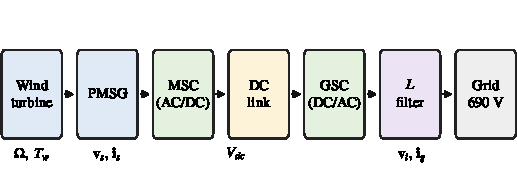
\includegraphics[width=\columnwidth]{system.pdf}
\caption{Direct-drive PMSG wind energy conversion system with a back-to-back converter.}
\label{fig:system}
\end{figure}

The power captured by the rotor and the tip-speed ratio are~\cite{heier2014,aimene2022}
\begin{equation}
P_w = \tfrac{1}{2}\rho\pi R^2 C_p(\lambda,\beta)\,v^3,\qquad \lambda=\frac{\Omega R}{v}
\label{eq:pw}
\end{equation}
where $\rho$ is the air density, $R$ the rotor radius, $v$ the wind speed, $\Omega$ the rotor speed and
$\beta$ the pitch angle. The power coefficient is
\begin{equation}
C_p = 0.5176\Bigl(\frac{116}{\lambda_i}-0.4\beta-5\Bigr)e^{-21/\lambda_i}+0.0068\lambda,
\label{eq:cp}
\end{equation}
with $1/\lambda_i=1/(\lambda+0.08\beta)-0.035/(\beta^3+1)$. For $\beta=0$, its maximum
$C_{p,\max}=0.48$ is reached at $\lambda_{opt}=8.1$ (Fig.~\ref{fig:turbine}). The aerodynamic torque is
$T_w=P_w/\Omega$.

\begin{figure}[t]
\centering
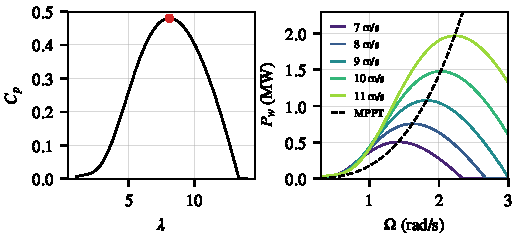
\includegraphics[width=\columnwidth]{turbine.pdf}
\caption{Power coefficient for $\beta=0$ (left) and captured power versus rotor speed for several wind
speeds, with the maximum power curve $P_{opt}=K_{opt}\Omega^3$ (right).}
\label{fig:turbine}
\end{figure}

For a rated power $P_n=2$~MW and $R=40$~m, a rotor radius typical of 2~MW turbines~\cite{rolan2009},
the rated wind speed follows from $P_n=\frac12\rho\pi R^2C_{p,\max}v_n^3$, which gives
$v_n=11.0$~m/s, and the rated rotor speed from $\Omega_n=\lambda_{opt}v_n/R=2.23$~rad/s. The rated
torque is $T_n=P_n/\Omega_n=0.897$~MN$\cdot$m. The maximum power curve is
$P_{opt}=K_{opt}\Omega^3$ with $K_{opt}=\frac12\rho\pi R^5C_{p,\max}/\lambda_{opt}^3$.

The direct-drive shaft is described by the one-mass model
\begin{equation}
J\frac{d\Omega}{dt} = T_w + T_e - B\Omega
\label{eq:shaft}
\end{equation}
where $J$ is the total inertia, $B$ the friction coefficient and $T_e$ the electromagnetic torque in
the receptor convention ($T_e<0$ in generating mode). The inertia is obtained by scaling the rotor
inertia of the 2~MW turbine of~\cite{van2015} ($6.3\times10^6$~kg$\cdot$m$^2$ for $R=45$~m) as
$J\propto R^5$, which gives $J\approx3.5\times10^6$~kg$\cdot$m$^2$ and an inertia constant
$H=J\Omega_n^2/(2P_n)=4.4$~s.

\section{Wind Speed Model}
Two wind profiles are used (Fig.~\ref{fig:wind}). The step profile (9, 11 and 8~m/s), similar to the
one of~\cite{aimene2022}, is used to assess the transient response. The turbulent profile combines a
mean value, low-frequency harmonics~\cite{regani2026} and a turbulence:
\begin{equation}
v(t) = V_m + \textstyle\sum_{k=1}^{3} A_k\sin(2\pi f_k t) + v_t(t)
\label{eq:wind}
\end{equation}
with $V_m=8.5$~m/s, $A=[1.5,\,0.2,\,0.3]$~m/s and $f=[0.03,\,0.16,\,0.17]$~Hz. The turbulence $v_t$
is a first-order coloured noise with a standard deviation of 0.5~m/s and a correlation time of
1.5~s, generated by a Park--Miller generator and the Box--Muller transform, so that the same sequence
is obtained on any platform. Over 40~s, the wind has a mean value of 8.6~m/s, a standard deviation of
1.1~m/s and remains between 6.0 and 10.9~m/s, i.e., below the rated wind speed, in the maximum power
point tracking region where the pitch angle is zero.

\begin{figure}[t]
\centering
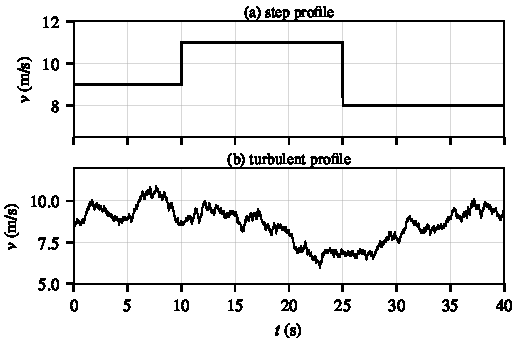
\includegraphics[width=\columnwidth]{wind.pdf}
\caption{Wind speed profiles: (a) steps of 9, 11 and 8~m/s; (b) turbulent profile (\ref{eq:wind}).}
\label{fig:wind}
\end{figure}

\section{PMSG Model}
In the rotor $dq$ frame (amplitude-invariant transformation, $d$ axis aligned with the magnet flux),
with the receptor convention and $L_d=L_q=L_s$, the PMSG is described by~\cite{aimene2022}
\begin{align}
v_{sd} &= R_s i_{sd} + L_s\frac{di_{sd}}{dt} - \omega_e L_s i_{sq}\label{eq:vsd}\\
v_{sq} &= R_s i_{sq} + L_s\frac{di_{sq}}{dt} + \omega_e L_s i_{sd} + \omega_e\psi_f\label{eq:vsq}\\
T_e &= \tfrac32 p\,\psi_f\, i_{sq}\label{eq:te}
\end{align}
where $\omega_e=p\Omega$, $p$ is the number of pole pairs and $\psi_f$ the magnet flux; in generating
mode, $i_{sq}<0$. With $\bv{i}_s=[i_{sd}\;i_{sq}]^T$, $\bv{v}_s=[v_{sd}\;v_{sq}]^T$, $\bv{e}_q=[0\;1]^T$
and the skew-symmetric matrix $\Jm=\bigl[\begin{smallmatrix}0&1\\-1&0\end{smallmatrix}\bigr]$,
\begin{equation}
L_s\dot{\bv{i}}_s = \bv{v}_s - R_s\bv{i}_s + \omega_eL_s\Jm\bv{i}_s - \omega_e\psi_f\bv{e}_q .
\label{eq:pmsg}
\end{equation}
The generator data are those of the non-salient 2~MW PMSG of~\cite{hasan2021} (Table~\ref{tab:param}).
At $\Omega_n$, the back-EMF $p\Omega_n\psi_f=532$~V is close to the peak phase voltage of the 690~V
grid (563~V), and the rated torque requires $i_{sq}=-T_n/(\frac32p\psi_f)=-2.51$~kA, consistent with
the rated current of about 2.6~kA given in~\cite{hasan2021}.

\begin{table}[t]
\caption{Parameters of the Studied System}
\label{tab:param}
\centering
\footnotesize
\setlength{\tabcolsep}{3pt}
\begin{tabular}{llll}
\toprule
Parameter & Symbol & Value & Source\\
\midrule
Rated power & $P_n$ & 2 MW & \cite{hasan2021}\\
Rotor radius & $R$ & 40 m & \cite{rolan2009}\\
Air density & $\rho$ & 1.225 kg/m$^3$ & \cite{aimene2022}\\
Rated wind / rotor speed & $v_n$, $\Omega_n$ & 11.0 m/s, 2.23 rad/s & (\ref{eq:pw})\\
Rated torque & $T_n$ & 0.897 MN$\cdot$m & $P_n/\Omega_n$\\
Total inertia & $J$ & $3.5\times10^6$ kg$\cdot$m$^2$ & \cite{van2015}\\
Friction coefficient & $B$ & $10^3$ N$\cdot$m$\cdot$s/rad & assumed\\
Pole pairs & $p$ & 26 & \cite{hasan2021}\\
Stator resistance & $R_s$ & 0.78 m$\Omega$ & \cite{hasan2021}\\
Stator inductance & $L_s$ & 1.57 mH & \cite{hasan2021}\\
Magnet flux & $\psi_f$ & 9.18 Wb & \cite{hasan2021}\\
DC-link capacitance & $C$ & 20 mF & \cite{hasan2021}\\
DC-link voltage & $V_{dc}$ & 1200 V & \cite{hasan2021}\\
Filter & $L_f$, $R_f$ & 0.15 mH, 2 m$\Omega$ & \cite{hasan2021}, assumed\\
Grid & & 690 V, 50 Hz & \cite{hasan2021}\\
Switching frequency & $f_{sw}$ & 2160 Hz & \cite{hasan2021}\\
\bottomrule
\end{tabular}
\end{table}

The model is first verified with the generator driven at $\Omega_n$ and connected to a balanced
resistive load of 0.19~$\Omega$ per phase ($\bv{v}_s=-R_L\bv{i}_s$). Fig.~\ref{fig:pmsg} shows that the
currents settle in about 40~ms to $i_{sd}=-1.08$~kA and $i_{sq}=-2.27$~kA. The electromagnetic torque is
negative ($-0.814$~MN$\cdot$m), i.e., it opposes the rotation, and the phase currents are balanced
sinusoids at the electrical frequency of 9.2~Hz. In steady state, the mechanical power absorbed by the
generator, 1.8144~MW, equals the power delivered to the load, 1.8069~MW, plus the copper losses,
7.4~kW, with a residual below $10^{-7}$~W.

\begin{figure}[t]
\centering
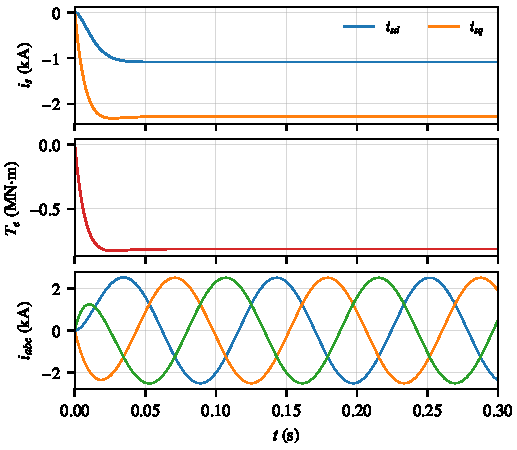
\includegraphics[width=\columnwidth]{pmsg.pdf}
\caption{PMSG driven at $\Omega_n$ and connected to a resistive load: $dq$ currents, electromagnetic
torque and phase currents $i_a$, $i_b$, $i_c$.}
\label{fig:pmsg}
\end{figure}

\section{Converter, DC Link and Grid Model}
The two-level converters are represented by their average model; the voltage vectors are limited to
$V_{dc}/\sqrt3$ (space-vector modulation). The DC link receives the power of the MSC and supplies the
GSC~\cite{aimene2022}:
\begin{equation}
CV_{dc}\frac{dV_{dc}}{dt} = P_{dc} - P_i,\quad P_{dc}=-\tfrac32\bv{v}_s^T\bv{i}_s,\quad
P_i=\tfrac32\bv{v}_i^T\bv{i}_g .
\label{eq:dc}
\end{equation}
In the grid-voltage-oriented frame ($v_{gq}=0$), the $L$ filter between the GSC voltage $\bv{v}_i$ and
the grid voltage $\bv{v}_g$, with the current $\bv{i}_g$ counted towards the grid, gives~\cite{aimene2022}
\begin{equation}
L_f\dot{\bv{i}}_g = \bv{v}_i - R_f\bv{i}_g + \omega_gL_f\Jm\bv{i}_g - \bv{v}_g ,
\label{eq:filter}
\end{equation}
and the grid powers are $P_g=\frac32v_{gd}i_{gd}$ and $Q_g=-\frac32v_{gd}i_{gq}$.

Equations (\ref{eq:shaft}), (\ref{eq:pmsg})--(\ref{eq:filter}) form a sixth-order model with state
$[i_{sd},i_{sq},\Omega,V_{dc},i_{gd},i_{gq}]$. With the stored energy
$E=\frac12J\Omega^2+\frac34L_s\|\bv{i}_s\|^2+\frac12CV_{dc}^2+\frac34L_f\|\bv{i}_g\|^2$, and since
$\bv{x}^T\Jm\bv{x}=0$ and $T_e\Omega=\frac32\omega_e\psi_fi_{sq}$, the model gives, for any state and
any converter voltages,
\begin{equation}
\dot E = P_w - B\Omega^2 - \tfrac32R_s\|\bv{i}_s\|^2 - \tfrac32R_f\|\bv{i}_g\|^2 - P_g .
\label{eq:balance}
\end{equation}
The aerodynamic power is thus stored, dissipated or delivered to the grid; this identity checks the
sign of every term of the model.

Table~\ref{tab:op} gives the operating point at $v=11$~m/s, with $\Omega$ at its optimal value,
$i_{sd}=0$ and unity power factor. The converter voltages remain below the limit
$V_{dc}/\sqrt3=693$~V. Simulated during 1~s with constant converter voltages, the model stays at this
equilibrium, and the power flow satisfies (\ref{eq:balance}) with a residual below $10^{-8}$~W.

\begin{table}[t]
\caption{Operating Point at $v=11$ m/s}
\label{tab:op}
\centering
\footnotesize
\setlength{\tabcolsep}{4pt}
\begin{tabular}{lll}
\toprule
Quantity & Symbol & Value\\
\midrule
Rotor speed & $\Omega$ & 2.228 rad/s\\
Stator / grid currents & $i_{sq}$, $i_{gd}$ & $-2460$ A, 2295 A\\
MSC / GSC voltages & $\|\bv{v}_s\|$, $\|\bv{v}_i\|$ & 575 V, 578 V\\
Aerodynamic power & $P_w$ & 1.967 MW\\
Friction / stator / filter losses & & 5.0 kW, 7.1 kW, 15.8 kW\\
Grid power & $P_g$ & 1.939 MW\\
\bottomrule
\end{tabular}
\end{table}

\section{Passivity-Based Current Control of the MSC}
With $\bv{e}_s=\bv{i}_s-\bv{i}_s^*$ and $\dot{\bv{z}}_s=\bv{e}_s$, the MSC voltage reference is
\begin{equation}
\bv{v}_s^* = L_s\dot{\bv{i}}_s^* + R_s\bv{i}_s^* - \omega_eL_s\Jm\bv{i}_s^* + \omega_e\psi_f\bv{e}_q
- R_a\bv{e}_s - K_i\bv{z}_s .
\label{eq:pbc}
\end{equation}
The first four terms reproduce the desired dynamics of (\ref{eq:pmsg}) along the reference, with the
coupling evaluated on the reference so that it remains workless; $R_a$ injects damping and $K_i$
removes the steady-state error. The reference derivative is obtained by a first-order filter (2~ms),
and the integral is frozen when $\|\bv{v}_s^*\|$ reaches $V_{dc}/\sqrt3$.

\begin{proposition}
With (\ref{eq:pbc}) applied to (\ref{eq:pmsg}) and $R_a,K_i>0$, the storage function
$H=\frac12L_s\|\bv{e}_s\|^2+\frac12K_i\|\bv{z}_s\|^2$ satisfies $\dot H=-(R_s+R_a)\|\bv{e}_s\|^2$ and
$\bv{e}_s\to0$.
\end{proposition}
\begin{proof}
Subtracting $L_s\dot{\bv{i}}_s^*$ from (\ref{eq:pmsg}) and inserting (\ref{eq:pbc}) gives
$L_s\dot{\bv{e}}_s=-(R_s+R_a)\bv{e}_s+\omega_eL_s\Jm\bv{e}_s-K_i\bv{z}_s$. Hence
$\dot H=\bv{e}_s^TL_s\dot{\bv{e}}_s+K_i\bv{z}_s^T\bv{e}_s=-(R_s+R_a)\|\bv{e}_s\|^2$, since
$\bv{e}_s^T\Jm\bv{e}_s=0$. $H$ is bounded and $\dot H$ is uniformly continuous, so Barbalat's
lemma~\cite{khalil2002} gives $\bv{e}_s\to0$.
\end{proof}

The gains place a double closed-loop pole at $\omega_i=500$~rad/s:
$R_s+R_a=2\omega_iL_s$ and $K_i=\omega_i^2L_s$, i.e., $R_a=1.569~\Omega$ and $K_i=392.5~\Omega$/s.

The controller is tested with the rotor speed held at $\Omega_n$. It is sampled at
$T_s=1/(2f_{sw})=231.5~\mu$s (regular sampling with double update), the voltage computed at one sample
is applied at the next one, and the plant is integrated with a fourth-order Runge--Kutta scheme. The
references are steps of $i_{sq}^*$ from 0 to $-1$~kA at 20~ms and to $-2.5$~kA (rated value) at 70~ms,
and of $i_{sd}^*$ from 0 to $-0.5$~kA at 120~ms (Fig.~\ref{fig:pbc}).

\begin{figure}[t]
\centering
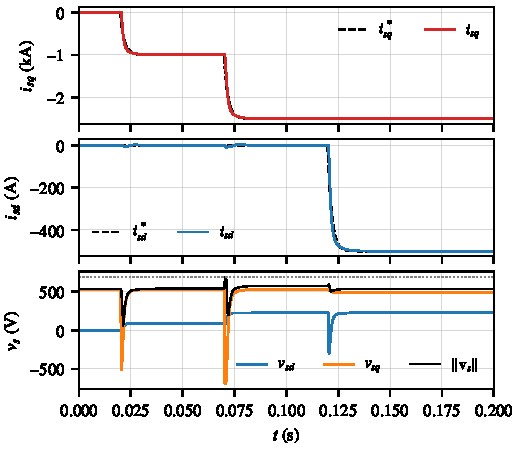
\includegraphics[width=\columnwidth]{pbc.pdf}
\caption{Passivity-based current control of the MSC at $\Omega=\Omega_n$: $q$- and $d$-axis currents
and their references, and stator voltages (dotted: limit $V_{dc}/\sqrt3$).}
\label{fig:pbc}
\end{figure}

\begin{table}[t]
\caption{Step Response of the Current Loop}
\label{tab:pbc}
\centering
\footnotesize
\begin{tabular}{ll}
\toprule
Indicator & Value\\
\midrule
Rise time (10--90\,\%), $i_{sq}$ step of $-1$ kA & 3.0 ms\\
Overshoot & 0\,\%\\
Maximum $|i_{sd}|$ during the $i_{sq}$ steps & 10.7 A\\
Steady-state error & 0 A\\
\bottomrule
\end{tabular}
\end{table}

Table~\ref{tab:pbc} summarizes the response. The currents follow their references with a rise time of
3~ms and no overshoot. The cross-coupling on $i_{sd}$ during the $i_{sq}$ steps is 10.7~A, i.e., about
0.4\,\% of the rated current, because the coupling terms are compensated in (\ref{eq:pbc}). The voltage
reaches the limit $V_{dc}/\sqrt3$ only during the step of $-1.5$~kA, where the reference derivative is
large; between the steps, $\|\bv{v}_s\|$ is about 575~V.

\section{Conclusion}
A 2~MW direct-drive PMSG wind energy conversion system was modeled from the turbine to the grid, with
generator, converter and grid data taken from published work and a turbine sized for the rated power.
The model is written in the receptor convention, and an exact power balance between the aerodynamic
power, the stored energy, the losses and the grid power verifies all its signs, both analytically and
numerically. Step and turbulent wind profiles were defined for the evaluation. A passivity-based
current controller for the machine-side converter, whose stability follows from a storage function,
tracks the current references with a rise time of 3~ms, no overshoot and a negligible cross-coupling,
with the sampling and the computation delay of a digital implementation. Future work will address the
speed control for maximum power point tracking, the DC-link and grid-current control of the grid-side
converter, and the compensation of parameter uncertainties.

\section*{Conflict of Interest}
The authors declare there are no conflicts of interest.

\begin{thebibliography}{99}
\bibitem{iea2024} International Energy Agency (IEA), \emph{World Energy Outlook 2024}, Paris, France, 2024.
\bibitem{gwec2024} Global Wind Energy Council (GWEC), \emph{Global Wind Report 2024}, Brussels, Belgium, 2024.
\bibitem{polinder2013} H. Polinder, J. A. Ferreira, B. B. Jensen, A. B. Abrahamsen, K. Atallah, and
R. A. McMahon, ``Trends in wind turbine generator systems,'' \emph{IEEE J. Emerg. Sel. Topics Power
Electron.}, vol.~1, no.~3, pp.~174--185, Sep. 2013.
\bibitem{wu2011} B. Wu, Y. Lang, N. Zargari, and S. Kouro, \emph{Power Conversion and Control of Wind
Energy Systems}. Hoboken, NJ, USA: Wiley-IEEE Press, 2011.
\bibitem{chinchilla2006} M. Chinchilla, S. Arnaltes, and J. C. Burgos, ``Control of permanent-magnet
generators applied to variable-speed wind-energy systems connected to the grid,'' \emph{IEEE Trans.
Energy Convers.}, vol.~21, no.~1, pp.~130--135, Mar. 2006.
\bibitem{yazdani2010} A. Yazdani and R. Iravani, \emph{Voltage-Sourced Converters in Power Systems:
Modeling, Control, and Applications}. Hoboken, NJ, USA: Wiley-IEEE Press, 2010.
\bibitem{mechter2016} A. Mechter, K. Kemih, and M. Ghanes, ``Backstepping control of a wind turbine for
low wind speeds,'' \emph{Nonlinear Dynamics}, vol.~84, no.~4, pp.~2435--2445, 2016.
\bibitem{messadi2015} M. Messadi, A. Mellit, K. Kemih, and M. Ghanes, ``Predictive control of a chaotic
permanent magnet synchronous generator in a wind turbine system,'' \emph{Chinese Phys. B}, vol.~24,
no.~1, Art.~no.~010502, 2015, doi: 10.1088/1674-1056/24/1/010502.
\bibitem{takhi2020} H. Takhi, K. Kemih, L. Moysis, \emph{et al.}, ``Passivity based control and
synchronization of perturbed uncertain chaotic systems and their microcontroller implementation,''
\emph{Int. J. Dyn. Control}, vol.~8, no.~3, pp.~973--990, 2020.
\bibitem{ortega1998} R. Ortega, A. Lor\'ia, P. J. Nicklasson, and H. Sira-Ram\'irez,
\emph{Passivity-Based Control of Euler-Lagrange Systems}. London, UK: Springer, 1998.
\bibitem{heier2014} S. Heier, \emph{Grid Integration of Wind Energy: Onshore and Offshore Conversion
Systems}, 3rd ed. Chichester, UK: Wiley, 2014.
\bibitem{aimene2022} M. Aimene, A. Payman, and B. Dakyo, ``Comparative study between flatness-based and
field-oriented control methods of a grid-connected wind energy conversion system,'' \emph{Processes},
vol.~10, no.~2, Art.~no.~378, 2022, doi: 10.3390/pr10020378.
\bibitem{hasan2021} S. M. M. Hasan and A. H. M. Shatil, ``Design and comparison of grid connected
permanent magnet synchronous generator non-salient pole and salient pole rotor wind turbine,''
\emph{AIUB J. Sci. Eng.}, vol.~20, no.~2, pp.~40--46, 2021.
\bibitem{rolan2009} A. Rolan, A. Luna, G. Vazquez, D. Aguilar, and G. Azevedo, ``Modeling of a variable
speed wind turbine with a permanent magnet synchronous generator,'' in \emph{Proc. IEEE Int. Symp. Ind.
Electron. (ISIE)}, Seoul, Korea, 2009, pp.~734--739, doi: 10.1109/ISIE.2009.5218120.
\bibitem{van2015} T. L. Van, T. D. Nguyen, T. T. Tran, and H. D. Nguyen, ``Advanced control strategy of
back-to-back PWM converters in PMSG wind power system,'' \emph{Adv. Electr. Electron. Eng.}, vol.~13,
no.~2, 2015, doi: 10.15598/aeee.v13i2.1161.
\bibitem{regani2026} S. Regani, M. Messadi, and K. Kemih, ``A novel chaos control approach with
adaptive ANN compensation for a DFIG-based wind turbine,'' \emph{Mathematics}, under review, 2026.
\bibitem{khalil2002} H. K. Khalil, \emph{Nonlinear Systems}, 3rd ed. Upper Saddle River, NJ, USA:
Prentice Hall, 2002.
\end{thebibliography}

\end{document}
